\documentclass[a4paper, twocolumn]{article}
\usepackage[pdftex, hidelinks]{hyperref}

\usepackage{bm}
\usepackage[T1]{fontenc}
\usepackage[utf8]{inputenc}
\usepackage{algorithmic}
\usepackage{algorithm}
\usepackage{amsfonts}
\usepackage{amssymb}
\usepackage{courier}
\usepackage{booktabs}
\usepackage{graphicx}
\usepackage{listings}
\usepackage{mathtools}
\usepackage{amssymb}
\lstset{basicstyle=\footnotesize\ttfamily,
        breakatwhitespace = false,
        breaklines = true,
        keepspaces = true,
        language = R,
        showspaces = false,
        showstringspaces = false,
        belowcaptionskip = \bigskipamount,
        framerule = 0.80pt,
        frame = tb,
        belowskip = \bigskipamount,
        escapeinside={<@}{@>}}

\title{TDDE01 -- Machine Learning \\
       Group 9 Laboration Report 3}
\author{{Martin Estgren \texttt{<mares480>}} \\
        {Erik S. V. Jansson \texttt{<erija578>}} \\
        {Sebastian Maghsoudi \texttt{<sebma654>}} \\~\\
        {Linköping University (LiU), Sweden}}

\begin{document}
    \pagenumbering{arabic}
    \maketitle % Generate.

    \section*{Assignment 1}

        In this assignment we are tasked with predicting the sex of Australian Crabs given their carapace length and the rear width. For this purpose we will be using
        Linear Discriminant Analyis (LDA) using Maximum Likelihood Estimation for predicting the unknown classification parameters. The first step involves plotting the
        data in order to determine if the data would be linearly separable into different categories (male and female in this case). This plot can be found in below in
        Figure~\ref{fig:crabs}.

        \begin{figure}
          \centering
          \caption{Sex Classification of Australian Crabs}
          \label{fig:crabs}
          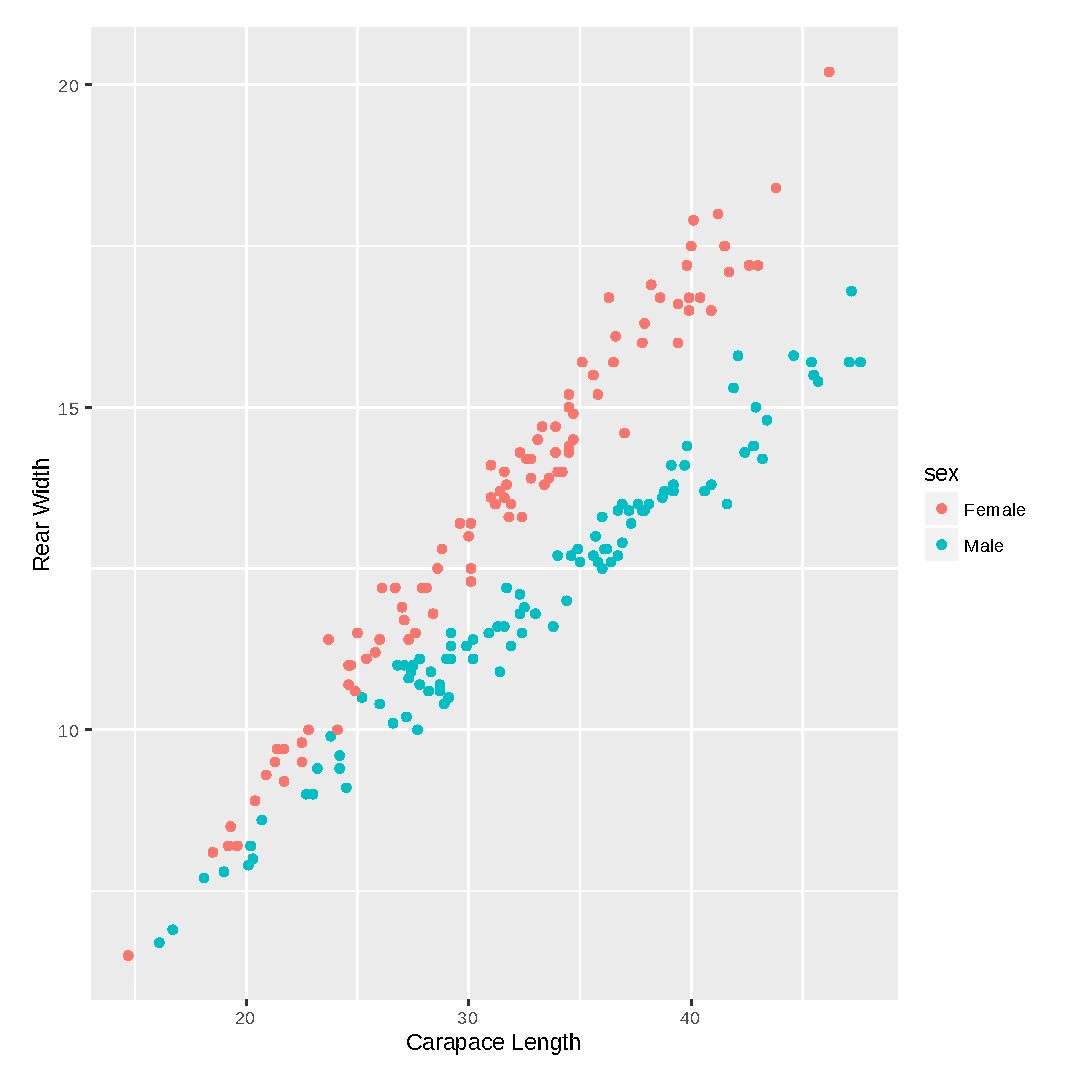
\includegraphics[width=0.5\textwidth]{share/crabs.eps}
        \end{figure}

        Our next task is to visualize the decision boundary between the different classifications. Since this is not already implemented by a package in R, we have to
        develop our own LDA method. A LDA can be implemented by comparing Linear Discriminant Functions (LDF) with each other, one for each corresponding class. In practice
        this means, since LDF is implemented with a likelihood function, one can assume that by applying predictor features to the function, the result would yield some indication
        of how likely this observation can be classified as the label corresponding to that LDF. An LDF can be described in the following way:

        \begin{equation} \label{eq:lda}
          \begin{split}
            \delta_k(x) &=  w_1 - b_1 \\
            w_1 &= x^{T}\Sigma^{-1}\mu_k, \\
            b_1 &= \frac{1}{2}\mu_k^{T}\Sigma^{-1}\mu_k+log\pi_k
          \end{split}
        \end{equation}

        After calculating the parameters for both labels (male and female) using the Equation~\ref{eq:lda} above, we can find the intercept and slope of the decision boundary
        separating both of these classes. This is done by simply subtracting each coefficient from each other, thereafter plotting this in Figure~\ref{fig:boundary}. Intuitively this
        is a short method of comparing likelihood of classes given feature predictors.     

        \begin{figure}
          \centering
          \caption{Sex Classification of Australian Crabs}
          \label{fig:boundary}
          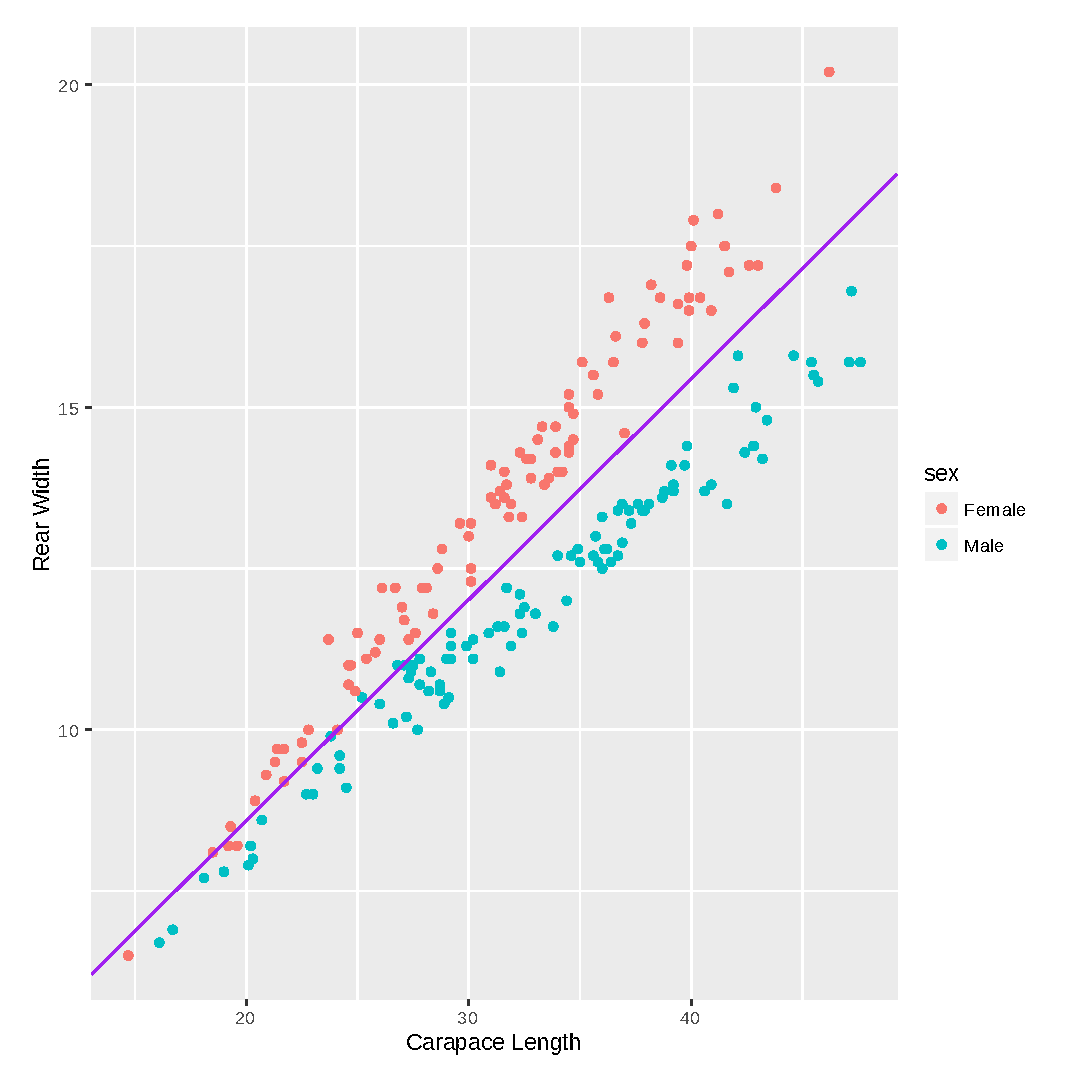
\includegraphics[width=0.5\textwidth]{share/boundary.eps}
        \end{figure}
       The final part is to compare the result received by implementing the LDA method with the result from using logistic regression. In r, there is package for this called \textit{glm}. 
	   The function \textit{glm()} returns a vector containing the coefficients including the intersection. The result can be seen in figure \ref{fig:LR}. Ass the observer can see, there 
	   is no significant difference between the result of the method, at least when it come to classify the sample observations. 

    \section*{Assignment 2}
	This assignment revolved around classification of the credit score of clients. The response depended on some other factors commonly linked with what lenders evaluate before giving credit. 
	The credit score of clients could be divided simply in good or bad.\newline
    The methods that is appropriate for this are prediction through a decision tree or a naive Bayesian model. The first model to evaluate is the decision tree. A decision tree simply create  
	model that depending on the value of some attributes can predict the response. The attributes is ranked in a tree form, where the more definitive attributes tend to be at the top. When the 
	the model is used for prediction the algorithm simply traverse the tree and following which path corresponds to the values for the corresponding attribute.

	The sample observations are randomly split into three parts with the size:
	\begin{equation}
		\left | testing \right | = \frac{\left | data \right |}{2}
	\end{equation}
	\begin{equation}
		 \left | training \right | = \frac{\left | data \right |}{4}
	\end{equation}
	\begin{equation}
	 \left | validation \right | = \frac{\left | data \right |}{4}
	\end{equation}

	\subsection{Decision tree}

	The \textit{training} set is used to train two decision tree models. One with \textit{deviance} and one with \textit{gini index} as metric. The resulting trees can be observed in the figures \ref{fig:deviance tree}/\ref{fig:gini tree} respectively.
	\begin{figure}
	    \centering
		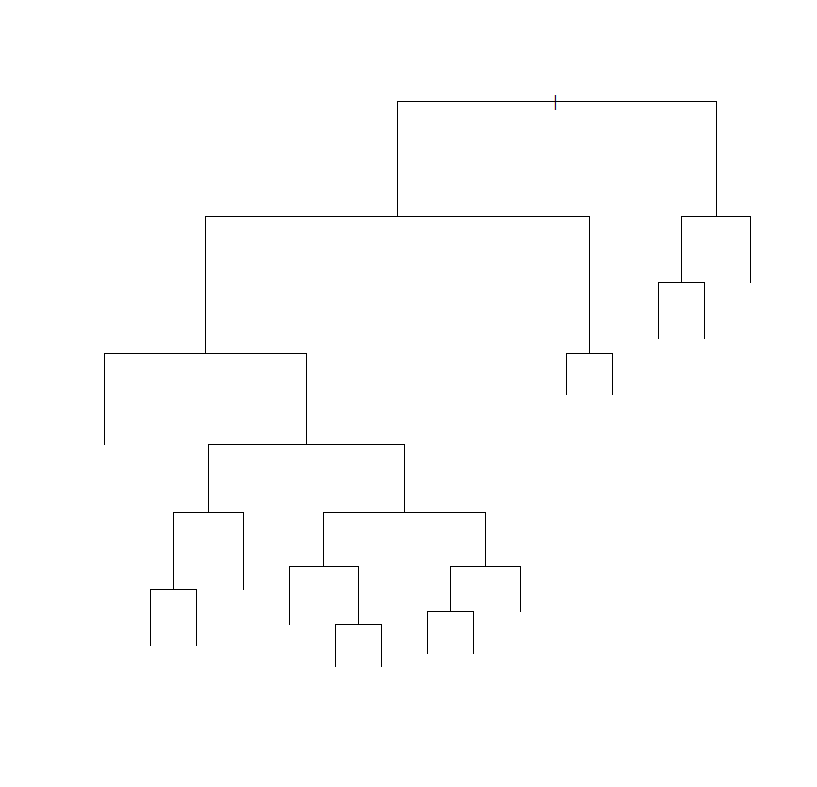
\includegraphics[width=0.5\textwidth]{share/deviance_tree.png}  
		\caption{\textit{Deviance} decision tree.\label{fig:deviance tree}}
	\end{figure}
	\begin{figure}
	    \centering
		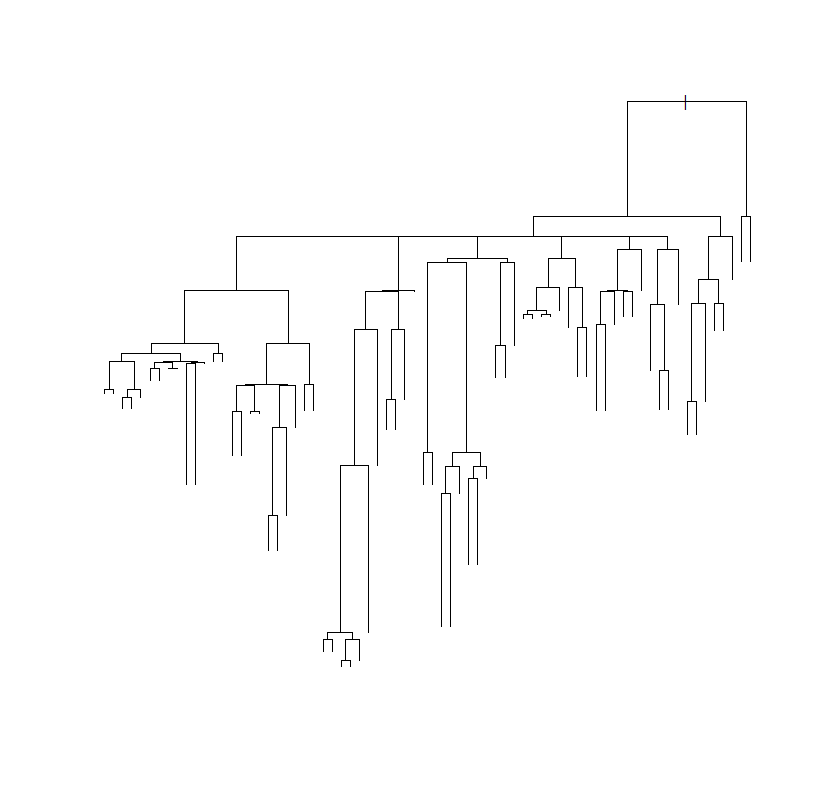
\includegraphics[width=0.5\textwidth]{share/gini_tree.png}  
		\caption{\textit{gini index} decision tree.\label{fig:gini tree}}
    \end{figure}
    The \textit{gini index} tree have significantly increased complexity compared to the \textit{deviance} and, when predicting the \textit{testing} data slightly higher misclassification rate.
	\begin{verbatim}
	deviance model fitness
	       predicted
	       bad good
	  bad   29   17
	  good  45  159
	misclassification rate: 0.248
	\end{verbatim}
	\begin{verbatim}
	gini model fitness
	       predicted
	       bad good
	  bad   24   26
	  good  50  150
	misclassification rate: 0.304
	\end{verbatim}
	The \textit{deviance} model is decided to be the better model.

	In order to determine the best max tree depth of the \textit{deviance} model we iterates through all depths between 2 and 15.
	\begin{figure}
	\centering
	\begin{minipage}[]{0.5\textwidth}
	  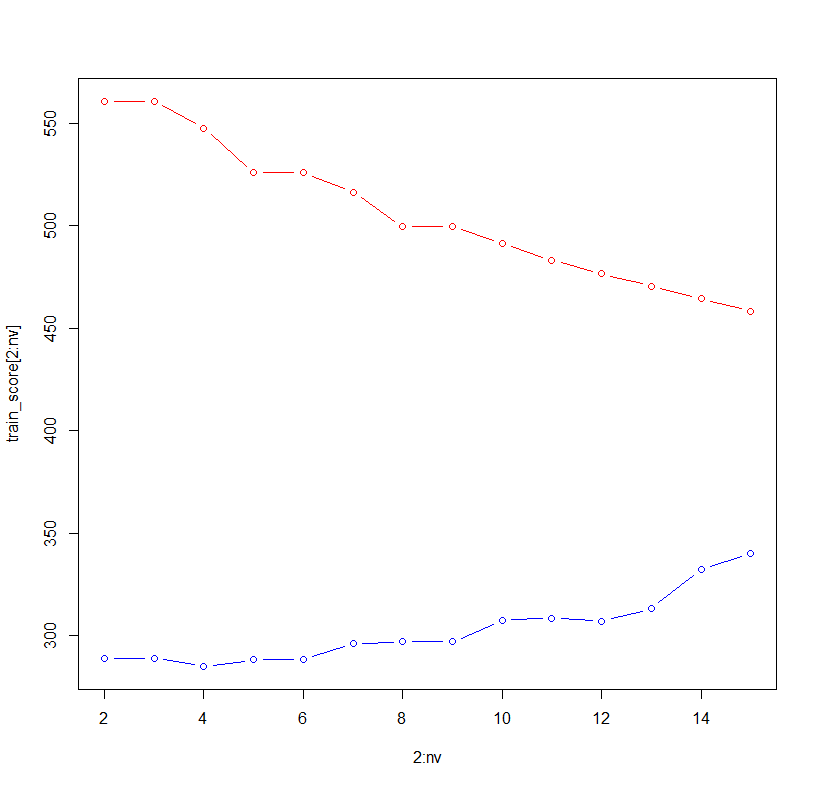
\includegraphics[width=\textwidth]{share/depth_tree.png}  
	  \caption{deviance for different max tree depths.\label{fig:tree_depth}}
	 \end{minipage}
	\end{figure}
	The \textit{red} line indicates deviance of the training data and the \textit{blue} line, the validation data. Tree depth of 4 results in the least deviance for the validation data. With a max tree depth of 4 the following classification table is produced.
	\begin{verbatim}
	optimal depth deviance fitness
	       predicted
	       bad good
	  bad   20   59
	  good   9  162
	misclassification rate: 0.272
	\end{verbatim}
	The misclassification rate is slightly lower than the \textit{gini index}. The tree is ploted in figure \ref{fig:best_subtree}.
	\begin{figure}
		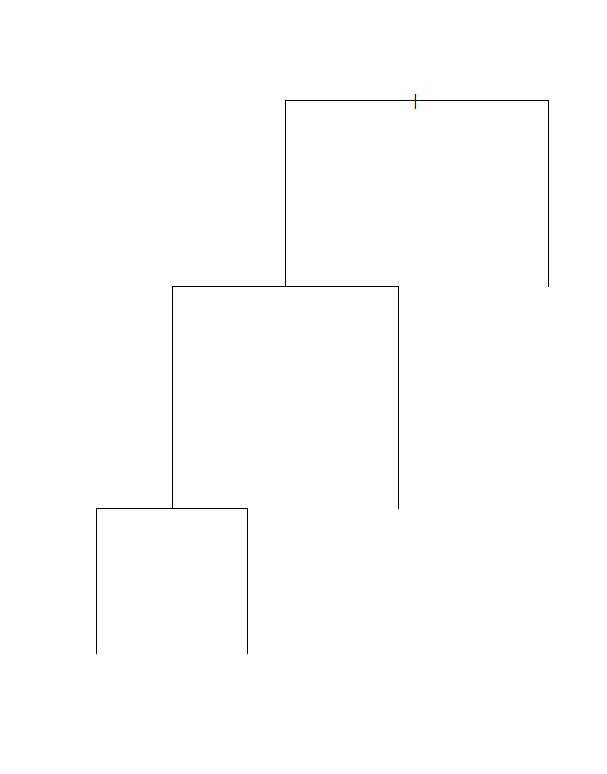
\includegraphics[width=0.5\textwidth]{share/best_subtree.png}  
		\caption{\textit{Deviance} decision tree at max depth 4.\label{fig:best_subtree}}
	\end{figure}

	\subsection{Naive Bayes}
    
    \nocite{*} % No warnings.
    \bibliographystyle{alpha}
    \bibliography{report}
    \onecolumn \appendix
    \section*{Appendix}

        ...

\end{document}
